\documentclass[a4paper,12pt]{article}
\setlength{\parskip}{1em}
\setlength{\parindent}{0em}
\usepackage[justification=centering, margin=2cm, labelfont=bf, font={small}]{caption}
\usepackage{float}
\usepackage{url}
\usepackage{subcaption}
\usepackage{tikz}
\usepackage{graphicx}
\usepackage{hhline}
\usetikzlibrary{shapes,arrows}


\begin{document}

\title{Refactoring and Reflection}
\author{Exam No. B024703}
\date{\today}
\maketitle

All sources described in this report are available from: 

\verb|https://github.com/jacobjwebber/software-development|

\section{Introduction}
This short report describes and reflects upon the work done in refactoring a small web application that facilitates the playing of a tabletop game. 

Development work was done according to Agile principles, with small user stories grouped into sprints and then completed. These individual stories or issues were stored and tracked using GitHub's tool for this purpose. The detail of these is not unnecessarily repeated here. Instead, this report provides an overview of the process, direction to where this further technical detail is documented, and a critical reflection on how successful this project was. This is followed by a brief conclusion.

\section{The Process}
\label{process}

The process was outlined to some extent in the \emph{Planning and Risks} (P+R) document. This section provides more detail as to how this was done on a technical level.

\subsection{Sprints and Sprint Planning}


\subsection{GitHub Issue Tracking}

\begin{figure}
\centering
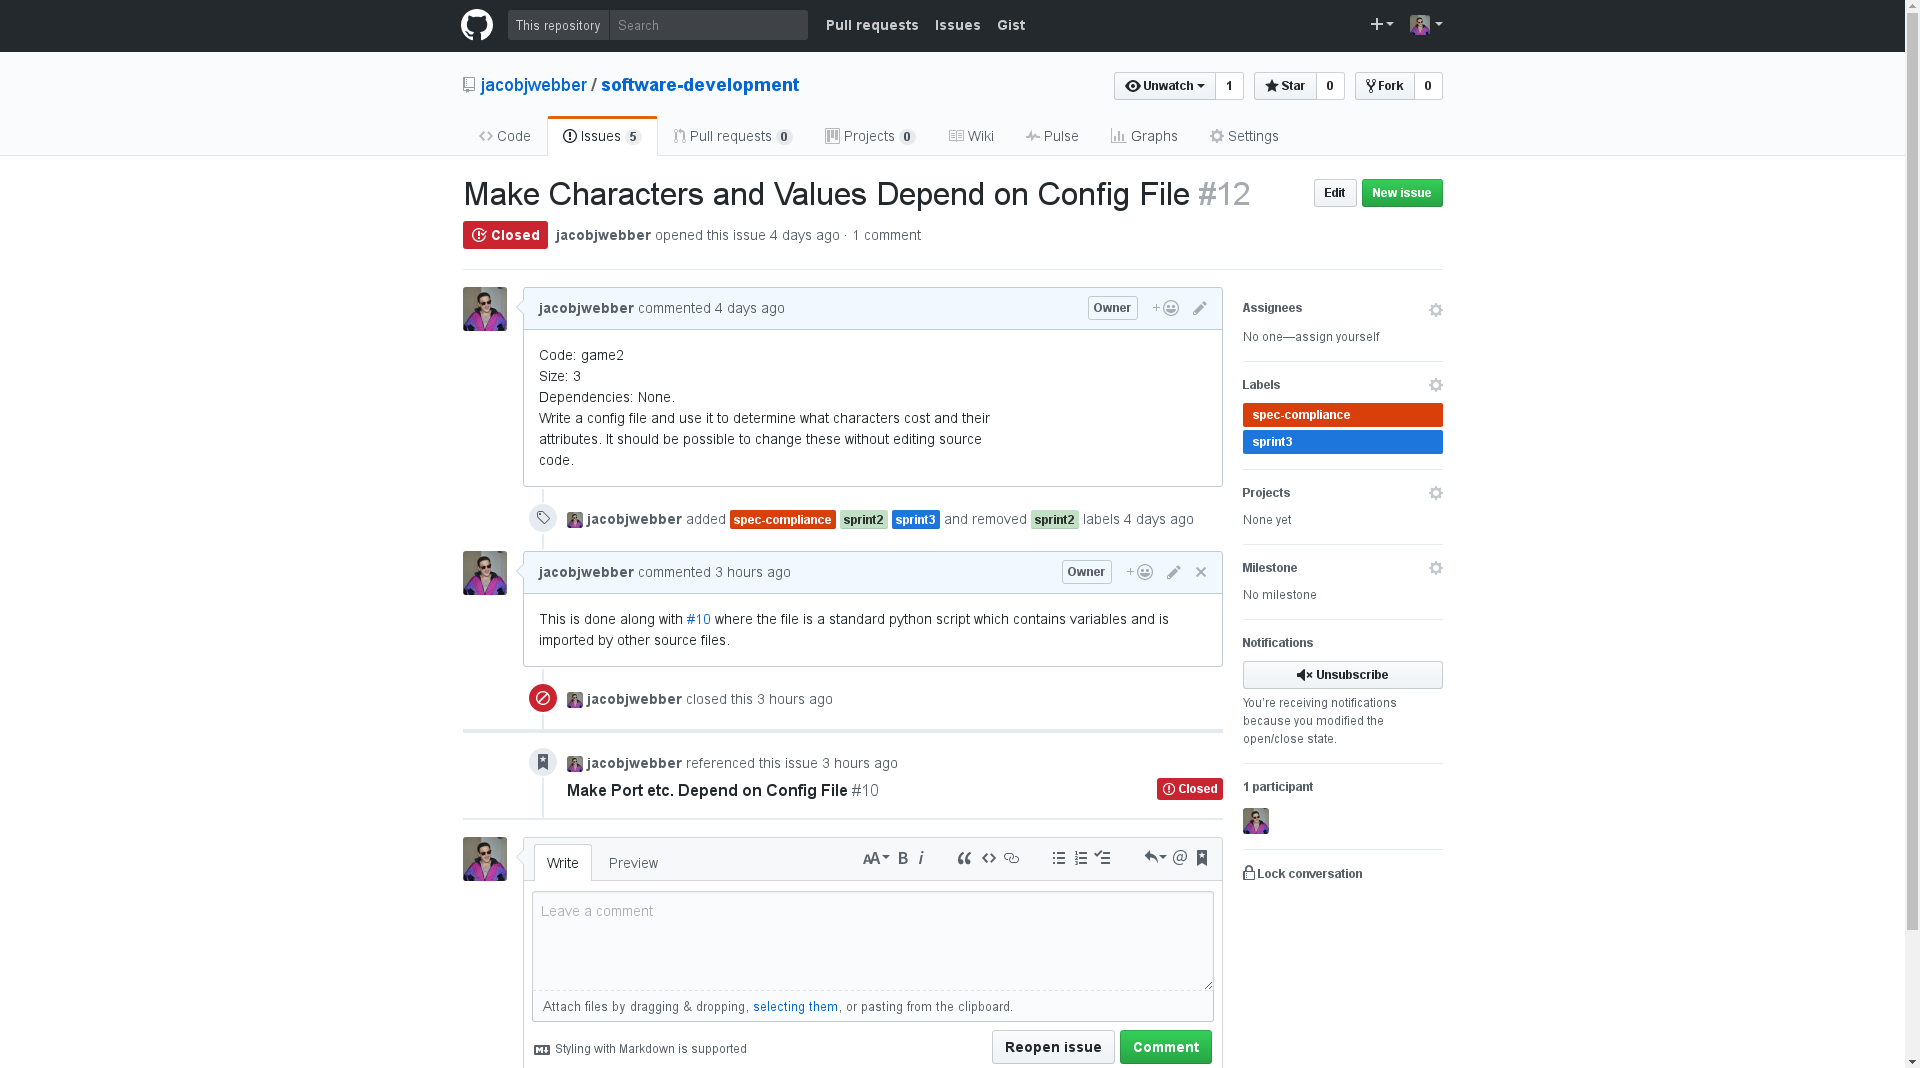
\includegraphics[width=\textwidth]{issue-screen}
\caption{Screen-shot of the issue tracking in GitHub}
\label{issuee}
\end{figure}

All of the issues discussed in P+R were uploaded to the GitHub issue tracking tool. These were marked according to their epic and according to what sprint they were in. Epics are particular genres of issues, such as bugs, and sprints were sections of work to be completed in one go. Only the issues that made up sprint 1 were determined in the P+R document, so new sprint planning sessions were done during the process. These sprint plans are also stored in the GitHub issue tracker. 

The issues in this form are very simple. They just allow a title and comments, as well as tags and the ability to be marked as open or closed. This was in general a positive, as the issues could be tagged with the appropriate sprint and epic, and marked as complete with no unnecessary complications. These issues can easily be searched for using these tags, so that the user can tell quickly, for example, how many issues are left in the current sprint. 

Figure \ref{issuee} shows this clearly. Note how the issue is marked as closed, but it is easy to see what sprint it was resolved as. GitHub allows the easy referencing of other issues which is used here to show that two issues were resolved together. As well as allowing easy organisation, this method of doing work provides complete documentation of the development process that any future developer could look at. This can help explain design decisions and contributes to a well documented source base with very little additional overhead.

These issues can be found at
\begin{verbatim}
https://github.com/jacobjwebber/software-development/issues
\end{verbatim}

To see those issues that have been closed, it is necessary to clear the search bar. These issues should be taken as documentation of all the work that has been completed.

\subsection{Git and Continuous Integration}
As the name suggests, Git is at the very core of GitHub. Git is a revision control system that allows a developer to track changes, revert and form branches. These features were used extensively throughout the development process. The initial branching strategy was to leave the original untouched on branch ``master'' and to form a new branch for development work called ``develop''. From this a new branch would be made for each issue tackled and then this would be merged back into ``develop'' when complete. However, this proved too time consuming, particularly when tackling smaller issues. Instead, only the very large issues followed this strategy, and all other work was done directly on branch ``develop''. Preserving the original code as received on branch ``master'' proved a useful reference for later work. Only when development work was completed was this pulled into the ``master'' branch.

The use of GitHub and Git also allowed for continuous integration to be done with Travis CI. Travis CI is a product from GitHub that runs builds on a server. These builds perform the unit tests as defined in the build script every time code is committed to GitHub. The tool also provides a build status that can be embedded in the project's home page, showing whether all tests are passing on each branch.

The source is published open source under the MIT license. A \verb|LICENSE.txt| file is included. 

\subsection{Debugging and Development}

\begin{figure}
\centering
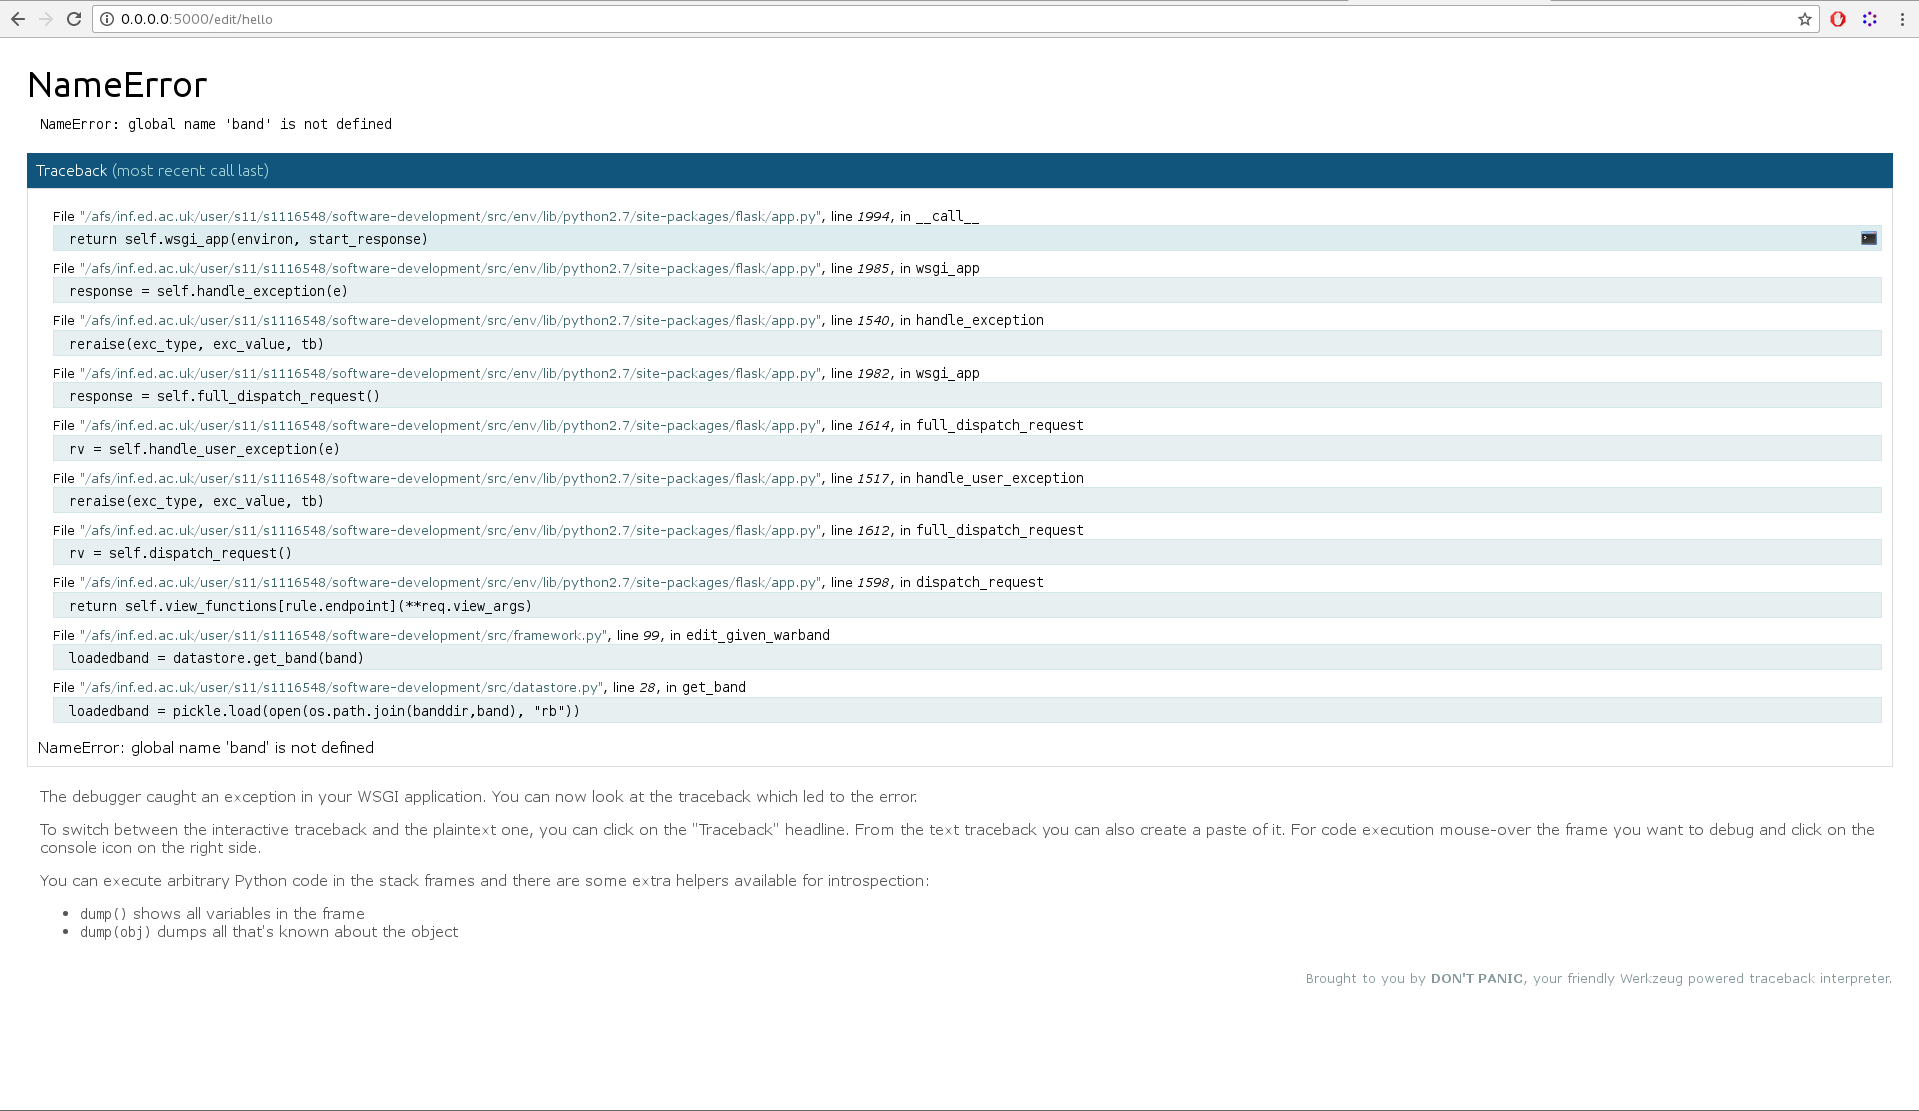
\includegraphics[width=\textwidth]{debug-screen}
\caption{Screen-shot of the debugging process with Flask's built in debugger}
\label{spr}
\end{figure}

The Flask framework provides a built in debugger. This can be activated by setting the environment variable \verb|FLASK_DEBUG| equal to 1. When there is a error in the Python source the browser window will show a full stack trace in an easy-to-read format. Figure \ref{spr} shows what this looks like when a standard bug is hit. Flask also allows for automatic reloading, so that the server updates itself when source files are modified.

\section{Reflection}

\subsection{Work Done}

While the reader can view the GitHub page and the list of issues contained for a full list of all tasks completed, this section provides at a higher level a picture of what work was selected, and why. This is contrasted with the work that was set out for completion in the P+R document.

As originally planned, the work done focusses on getting the code into a good state rather than adding functionality, or fixing issues of specification compliance. This meant heavily refactoring the code by abstracting away repeated code into separate functions, and breaking suitable pieces into separate python modules. These modules were then extensively unit tested. Additionally, as laid out in P+R, little work was done on improving the user interface. This was deemed out of scope of this particular section of work. This is because redesigning this user interface needs to happen from the ground up, with the collaboration of the customer and the end users. This process is set out in the \emph{UI	and	Evaluation	Plan} document included. It did not seem appropriate to waste time fixing a very limitted UI when this work is going to go ahead. 

Beyond this, a very pragmatic reason for not undertaking this work is the fact that a significant amount of time would have been required researching the use of HTML and JavaScript for a developer who only has experience in back end technologies. As discussed in \ref{eval}, the process of learning Python to a suitable level took a very large chunk of the total project time, repeating this endeavour for these front end technologies would not have been practical. This means that, while the back end code is much cleaner, several serious bugs in the user interface remain. Examples include the inability to submit edits to the squads, incorrect labelling of game features and a very unpleasant to use interface.

As described in section \ref{process}, much of the work done in this project when into gathering the necessary skills and establishing a good, professional process. This means that a system of source control, issue tracking and continuous integration is now well implemented which will make all future work much easier to complete. The added bonus of completing this less visible work first is that it will not unduly raise customer expectations, as would be the case if quick wins were prioritised over the abolition of technical debt.

\subsection{Evaluation}
\label{eval}

As predicted in the P+R document, developer inexperience did prove to be a risk and indeed one that was realised. This meant that a great deal of time was spent on becoming proficient enough in Python for development work to begin. This process took at least a week longer than expected, severely delaying other work.

The developer also had a period of sickness which impacted on this work. This was not marked as a risk in the P+R document, which was probably a mistake. This negative outcome was exacerbated by the fact that this was not the only project being worked on by the developer, meaning complex time management was displaced by the period of sickness and the developer had to balance catching up with all projects simultaneously.

However, the developer was still able to devote some serious time to this project. This ended up being in the form of about 1.5 weeks full time, as opposed to the 3 part time weeks plus learning time originally scheduled. 3 full sprints as outlined in P+R were still completed, as well as almost all issues outlined in that document. The code is undeniably very much cleaner, easier to read and easier to work on, and all further work will be greatly assisted by the additional tooling provided.

It is disappointing it was not possible to do more to make the application better for the user, and particularly disappointing that the user interface is not fully functional. In the end the developer simply did not have the skills to fix bugs in the front end code. In addition, illness and the time taken to learn Python meant adding functionality was not possible. While some justification has been given as to why clean and well tested code was prioritised instead of these improvements, the balance was probably too far against improving functionality and too much towards best practice. 

\subsection{Future Enhancement}

The application still has a very limitted user interface which is riddled with bugs. This needs to be fully redesigned and re-engineered. To do this it is recommended that a developer with front end experience is found, or that time is allowed for the gathering of these skills. The process by which the front end redesign might happen is outlined in the \emph{UI	and	Evaluation	Plan} document.

In addition to this, none of the multi-user features defined by the specification have been implemented, including a log-in process or the ability to share squads. This process will be a complex one to engineer, which should be emphasised to the customer. The customer should then decide if they have the necessary resources to complete this work.

It is critical that before future work is done, the current state of the application is discussed with the client to verify what the correct outcome is, as well as what customer priorities are. This was the reason why, for example, the game terminology as mentioned in the specification was not implemented. The application as received used different terminology from this, for example ``Wizard'' became ``Captain'', but it was not known which of these was correct. Treating a specification as a single point of truth will often yield bad outcomes and inflexibility. 

\section{Conclusion}
To conclude, a significant amount of work was done to improve the supplied application. This included cleaning the code, refactoring it to make it into appropriate modules and writing a suite of unit tests. In addition, appropriate tooling was selected and implemented, such as GitHub source control, Travis CI and GitHub issues.

However, the project was not a great success. No new functionality was added, mainly due to illness and the developer's unfamiliarity with Python. While this was disappointing, the changes that were made and tooling introduced will make all of this work much easier to accomplish in the future.


\end{document}